\documentclass{article}
\usepackage{amsmath}
\usepackage{hyperref}
\usepackage{graphicx}
\usepackage{minted}
\usepackage[UTF8]{ctex}

\hypersetup{
  colorlinks=true,
  allcolors=blue,
  pdfstartview=Fit,
  breaklinks=true
}

\begin{document}
  \title{系统开发工具基础 \\ 第一周实验报告}
  \author{乔海轩—25090012035}
  \date{2026年8月24日}
  \maketitle
  
  \tableofcontents
  \newpage

  \section{总览}
    \begin{table}[h]
      \centering
      \begin{tabular}{|l|l|c|}
        \hline
        题目编号 & 描述 & 完成情况 \\
        \hline
        1 & 含空格文件名的批量整理 & 已完成 \\
        2 & 随机访问日志统计 & 已完成 \\
        3 & 制造、解决并解释一次合并冲突 & 已完成 \\
        4 & 修复并构建一页技术说明 & 已完成 \\
        \hline
      \end{tabular}  
    \end{table}
    Github 仓库地址：\href{https://github.com/Ptilotsis-o/system-dev-tools/}{https://github.com/Ptilotsis-o/system-dev-tools/}
    \newline Commit记录如图\ref{fig:commit}所示。
    \begin{figure}[h]
      \centering
      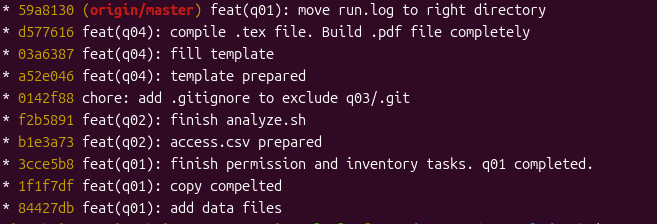
\includegraphics[width=0.8\textwidth]{figures/commit.png}
      \caption{Commit记录截图}
      \label{fig:commit}
    \end{figure}
  
  \newpage
  \section{第 1 题 含空格文件名的批量整理}
    \subsection*{题目要求}
      \begin{itemize}
        \item 创建 input/docs 和 input/tmp；
        \item 创建 input/docs/notes one.txt（内容为 alpha 和 beta 两行）、input/docs/.secret.txt（内容为 hidden）、input/tmp/empty.txt（空文件）以及 input/run.log（任意两行日志）。
        \item 显示 q01 的绝对路径，并以长格式列出 input 下全部项目，包含隐藏文件。
        \item 把 input 下所有.txt 文件复制到 work/学号/，保留相对目录结构并正确处理名称中的空格。
        \item 将复制后的目录权限设为 750、普通文件权限设为 640；生成 inventory.txt，列出相对路径和字节数。
      \end{itemize}
    \subsection*{操作步骤与命令}
      \begin{minted}{bash}
        mkdir -p input/docs input/tmp
        echo -e "alpha\nbeta" > input/docs/"notes one.txt"
        echo "hidden" > input/docs/.secret.txt
        touch input/tmp/empty.txt
        echo "2026-08-24 15:00:00 Task started" > input/run.log
        echo "2026-08-24 15:03:00 Task finished" >> input/run.log
        pwd
        ls -la -R input
        mkdir -p work/25090012035/
        cp --parents input/docs/{*, .* }.txt input/tmp/{*, .* }.txt work/25090012035/
        find work/25090012035 -type d -exec chmod 750 {} \;
        find work/25090012035 -type f -exec chmod 640 {} \;
        find . -type f -printf "%P %s\n" > inventory.txt
      \end{minted}
    \subsection*{结果验证}
      \begin{itemize}
        \item 绝对路径显示正确；
        \item input 下全部项目已列出，包含隐藏文件；
        \item work/25090012035 下的文件已正确复制，目录结构保持不变，空格处理正确；
        \item 权限设置正确，目录为 750，普通文件为 640；
        \item inventory.txt 列出了相对路径和字节数。
      \end{itemize}
      \begin{figure}[h]
        \centering
        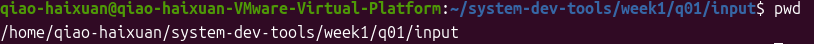
\includegraphics[width=0.8\textwidth]{figures/pwd.png}
        \caption{pwd截图}
        \label{fig:pwd}
      \end{figure}
      \begin{figure}[h]
        \centering
        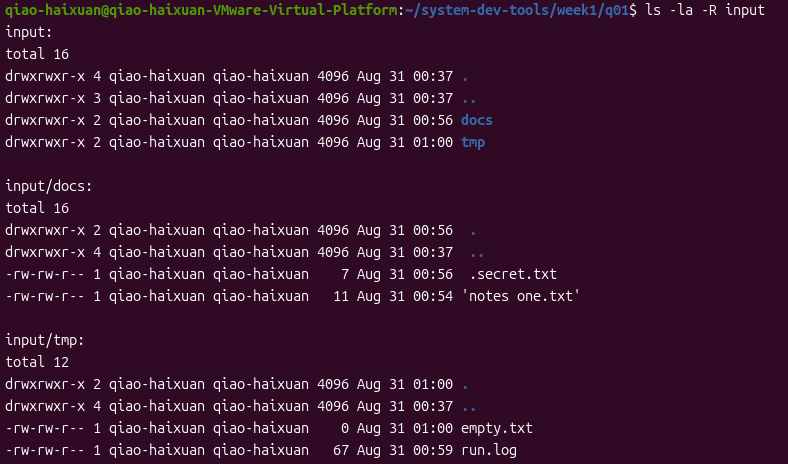
\includegraphics[width=0.8\textwidth]{figures/ls.png}
        \caption{ls -la -R input截图}
        \label{fig:ls}
      \end{figure}
      \begin{figure}[h]
        \centering
        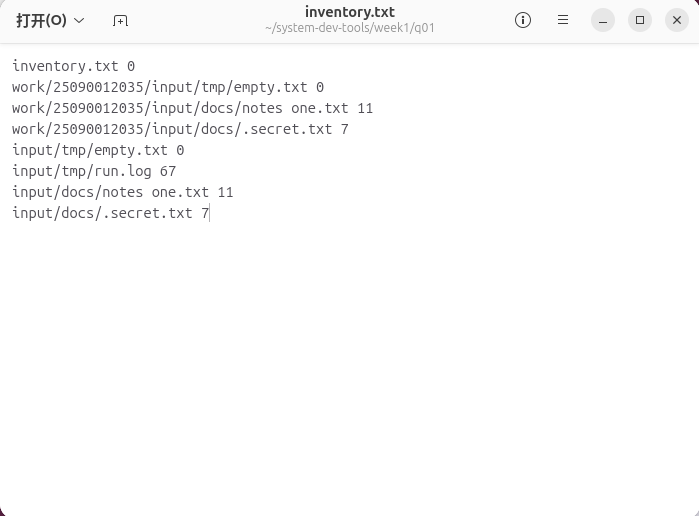
\includegraphics[width=0.8\textwidth]{figures/inventory.png}
        \caption{inventory.txt截图}
        \label{fig:inventory}
      \end{figure}
  
  \newpage
  \section{第 2 题 随机访问日志统计}
    \subsection*{题目要求}
      \begin{itemize}
        \item 编写 analyze.sh，接收一个 CSV 文件路径；文件不存在时将错误写入 stderr 并返回非零退出码。
        \item 使用 Shell 管道以及 awk、sort、head 等工具，输出 HTTP 5xx 数量最多的前 2 个 path；按次数降序，次数相同时按 path 字典序。
        \item 输出全部数据行的平均 latency\_ms，保留两位小数；表头不得计入。
        \item 分别对 access.csv 和一个不存在的文件运行脚本；不得使用 Python、电子表格或手工统计。
      \end{itemize}
    \subsection*{操作步骤与命令}
      \begin{minted}{bash}
        vim analyze.sh
        chmod +x analyze.sh
        ./analyze.sh access.csv
        ./analyze.sh null.csv
        echo $?
      \end{minted}
    \subsection*{结果验证}
      \begin{itemize}
        \item analyze.sh 编写完成；
        \item analyze.sh 对 access.csv 运行，输出正确结果；
        \item analyze.sh 对不存在的文件运行，正确输出错误信息并返回非零退出码。
      \end{itemize}
      \begin{figure}[h]
        \centering
        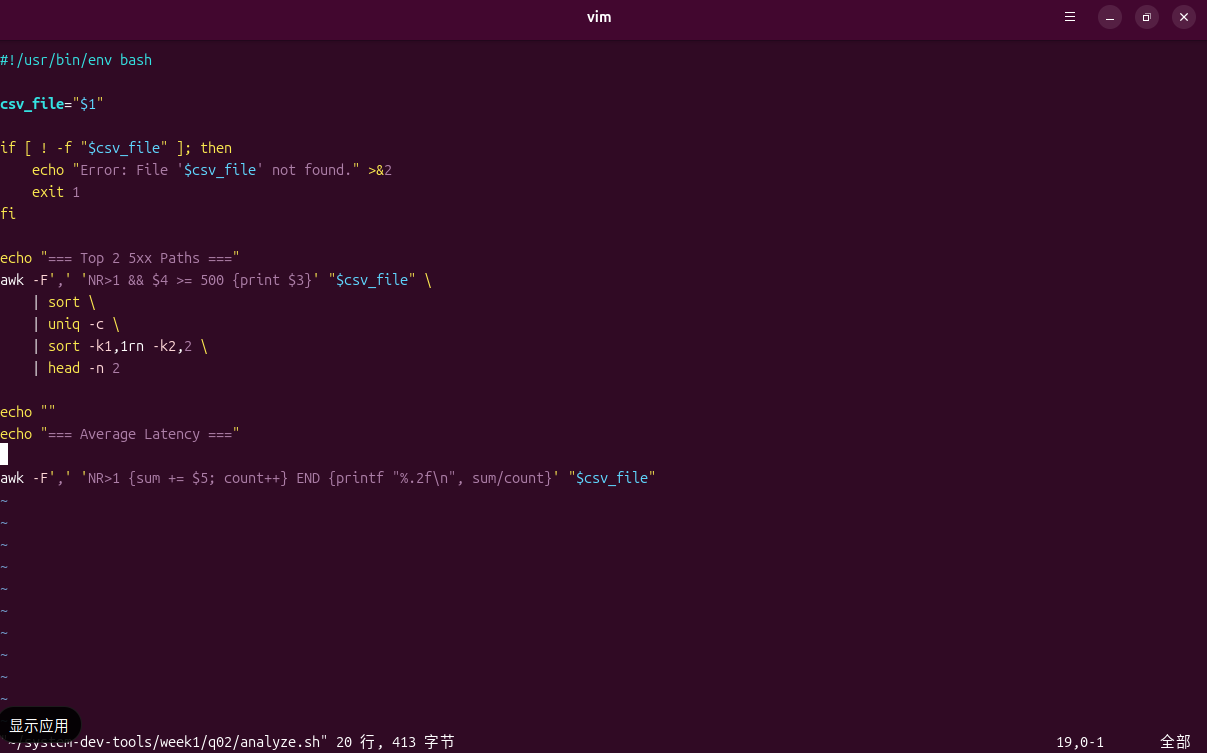
\includegraphics[width=0.8\textwidth]{figures/analyze.png}
        \caption{analyze.sh截图}
        \label{fig:analyze}
      \end{figure}
      \begin{figure}[h]
        \centering
        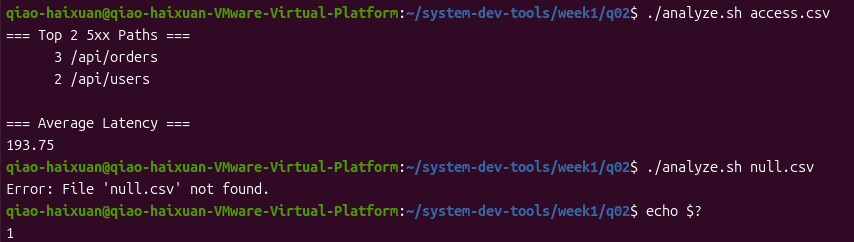
\includegraphics[width=0.8\textwidth]{figures/analyze_output.png}
        \caption{analyze.sh输出截图}
        \label{fig:analyze_output}
      \end{figure}
   
  \newpage    
  \section{第 3 题 制造、解决并解释一次合并冲突}
    \subsection*{题目要求}
      \begin{itemize}
        \item 初始化仓库，在 main 创建 config.txt，内容为 mode=normal，并完成初始提交。
        \item 创建 feature-a，把内容改为 mode=safe 并提交；从初始 main 创建 feature-b，把内容改为 mode=fast 并提交。
        \item 回到 main，先合并 feature-a，再合并 feature-b；解决冲突时保留 mode=safe，并另加一行 note=reviewed。
        \item 确认工作区干净，运行 git log --all --graph --decorate --oneline 查看历史。
      \end{itemize}
    \subsection*{操作步骤与命令}
      \begin{minted}{bash}
        git init
        echo "mode = normal" > config.txt
        git add config.txt
        git commit -m "Initial commit"
        git checkout -b feature-a
        echo "mode = safe" > config.txt
        git add config.txt
        git commit -m "change mode to safe"
        git checkout master
        git checkout -b feature-b
        echo "mode = fast" > config.txt
        git add config.txt
        git commit -m "change mode to fast"
        git checkout master
        git merge feature-a
        git merge feature-b
        git add config.txt
        git commit -m "merge feature-b: keep safe mode and add reviewed note"
        git status
        git log --all --graph --decorate --oneline
      \end{minted}
    \subsection*{结果验证}
      \begin{itemize}
        \item 仓库初始化完成，config.txt 创建并提交；
        \item feature-a 和 feature-b 分支创建并提交修改；
        \item 合并 feature-a 成功，合并 feature-b 时产生冲突，解决冲突后提交；
        \item 工作区干净，git log 输出显示分支合并历史。
      \end{itemize}
      \begin{figure}[h]
        \centering
        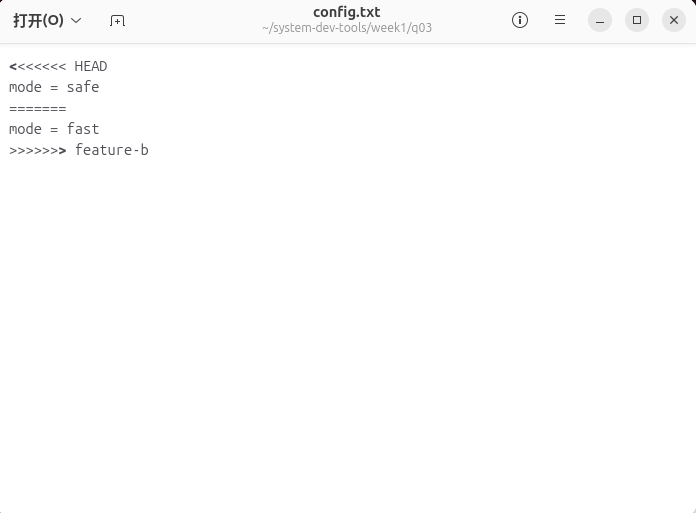
\includegraphics[width=0.8\textwidth]{figures/conflict.png}
        \caption{冲突发生时的 config.txt 内容截图}
        \label{fig:conflict}
      \end{figure}
      \begin{figure}[h]
        \centering
        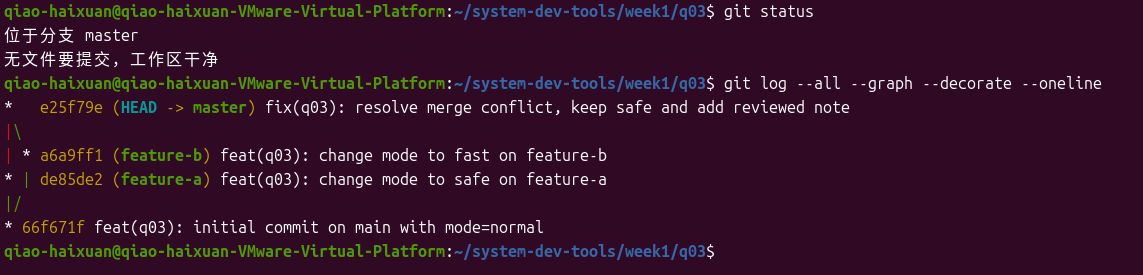
\includegraphics[width=0.8\textwidth]{figures/reviewed.png}
        \caption{git status 和 git log --all --graph --decorate --oneline  输出截图}
        \label{fig:reviewed}
      \end{figure}
  
  \newpage
  \section{第 4 题 修复并构建一页技术说明}
    \subsection*{题目要求}
      \begin{itemize}
        \item 加入一个带编号和 label 的公式，并在正文中使用 ref 或 eqref 引用。
        \item 加入一个 2 行 2 列表格，设置 caption 和 label，并在正文中引用该表。
        \item 使用 latexmk -pdf -halt-on-error 或 tectonic 生成 report.pdf。
        \item 确认 PDF 能打开，且交叉引用不显示“??”。
      \end{itemize}
      \subsection*{操作步骤与命令}
        \begin{minted}{bash}
          vim report.tex
          latexmk -xelatex -pdf -halt-on-error report.tex
        \end{minted}
      \subsection*{结果验证}
        \begin{itemize}
          \item 报告生成完成，PDF 能打开，交叉引用正常。
        \end{itemize}
        \begin{figure}[h]
          \centering
          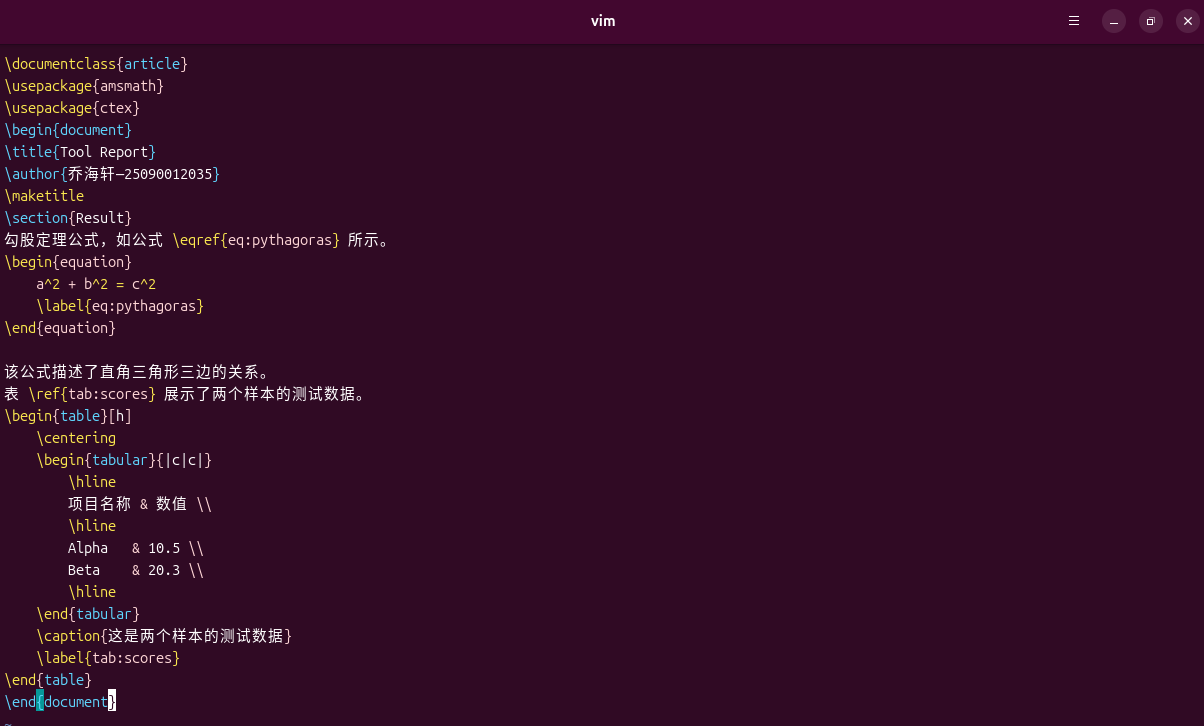
\includegraphics[width=0.8\textwidth]{figures/tex.png}
          \caption{report.tex截图}
          \label{fig:tex}
        \end{figure}
        \begin{figure}[h]
          \centering
          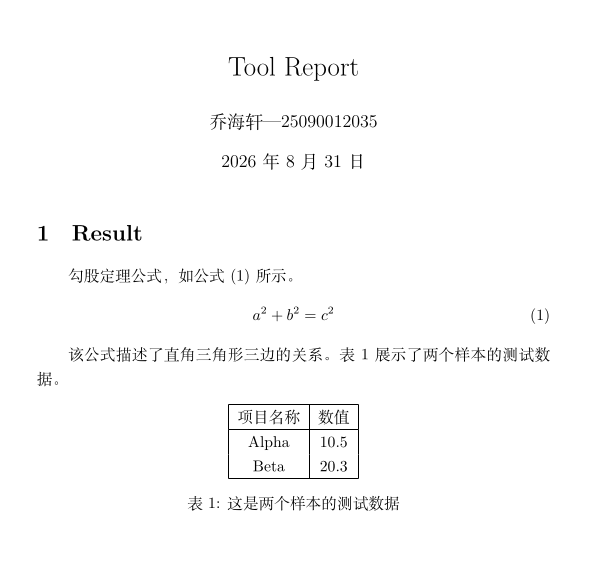
\includegraphics[width=0.8\textwidth]{figures/pdf.png}
          \caption{report.pdf截图}
          \label{fig:pdf}
        \end{figure}
  
  \newpage
  \section{课后作业}
    \subsection{q1: 批量删除空文件}
    目标：删除当前目录下所有大小为 0 字节的普通文件
      \begin{minted}{bash}
        find . -type f -size 0 -delete
      \end{minted}
    \subsection{q2: 批量重命名}
    目标：将当前目录下所有 .htm 文件重命名为 .html。
      \begin{minted}{bash}
        for f in *.htm; do mv "$f" "${f%.htm}.html"; done
      \end{minted}
    \subsection{q3: 统计子目录占用并按大小排序}
    目标：计算当前目录下所有子目录的磁盘占用，以人类可读方式显示，并按大小降序排列
      \begin{minted}{bash}
        du -sh */ | sort -hr
      \end{minted}
      \begin{figure}[h]
        \centering
        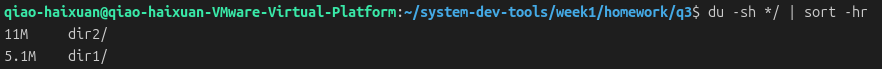
\includegraphics[width=0.8\textwidth]{figures/du.png}
        \caption{du -sh */ | sort -hr 输出截图}
        \label{fig:du}
      \end{figure}
    \subsection{q4: 统计词频并输出前3}
    目标：统计 article.txt 中每个单词出现次数，输出次数最多的前 3 个单词。
      \begin{minted}{bash}
        tr -s '[:space:]' '\n' < article.txt | sort | uniq -c | sort -nr | head -3
      \end{minted}
      \begin{figure}[h]
        \centering
        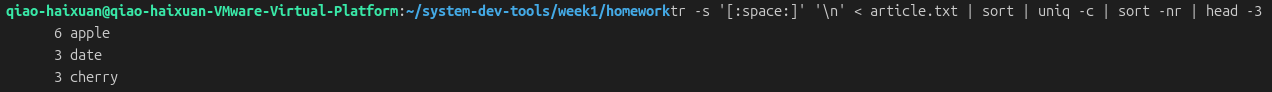
\includegraphics[width=0.8\textwidth]{figures/word.png}
        \caption{统计 article.txt 中每个单词出现次数，输出次数最多的前 3 个单词}
        \label{fig:word}
      \end{figure}
    \subsection{q5: 条件过滤并输出行号}
    目标：筛选 server.log 中包含日期 2026-08-24 且状态码为 404 的行，并在行首显示行号
      \begin{minted}{bash}
      grep -n '2026-08-24.*404' server.log
      \end{minted}
      \begin{figure}[h]
        \centering
        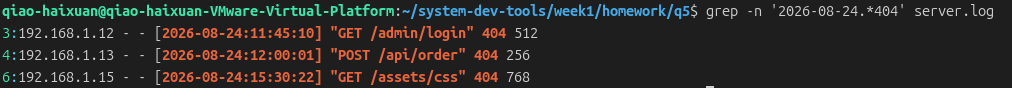
\includegraphics[width=0.8\textwidth]{figures/grep.png}
        \caption{grep -n '2026-08-24.*404' server.log 输出截图}
        \label{fig:grep}
      \end{figure}
    \subsection{q6: 两文件求交集并排序}
    目标：输出同时出现在 list1.txt 和 list2.txt 中的用户名，按字典序排列
      \begin{minted}{bash}
        comm -12 <(sort list1.txt) <(sort list2.txt)
      \end{minted}
      \begin{figure}[h]
        \centering
        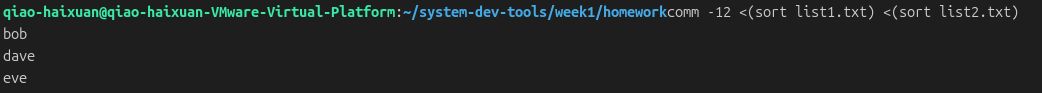
\includegraphics[width=0.8\textwidth]{figures/intersect.png}
        \caption{comm -12 <(sort list1.txt) <(sort list2.txt) 输出截图}
        \label{fig:intersect}
      \end{figure}
    \subsection{q7: 暂存未跟踪文件并恢复}
    目标：临时保存工作区所有修改（含新创建的未跟踪文件），清空工作区，随后恢复
      \begin{minted}{bash}
        git stash push -u
        git stash pop
      \end{minted}
      \begin{figure}[h]
        \centering
        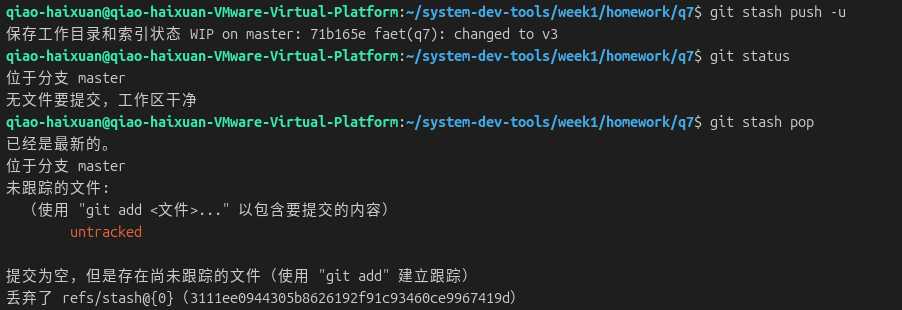
\includegraphics[width=0.8\textwidth]{figures/stash.png}
        \caption{git stash push -u 输出截图}
        \label{fig:stash}
      \end{figure}
    \subsection{q8: 修改最近一次提交信息}
    目标：修改最近一次提交的日志信息，不改变文件改动
      \begin{minted}{bash}
        git commit --amend -m "message changed"
      \end{minted}
    \subsection{q9: 查看特定文件的提交演变史}
    目标：仅显示 config.yml 的每一次提交变动摘要（不显示其他文件）
      \begin{minted}{bash}
        git log --oneline --follow config.yml
      \end{minted}
      \begin{figure}[h]
        \centering
        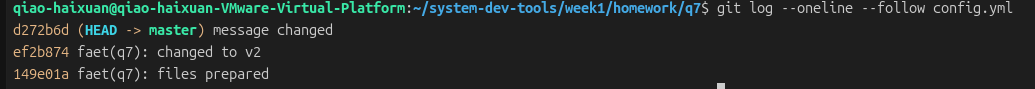
\includegraphics[width=0.8\textwidth]{figures/log.png}
        \caption{git log --oneline --follow config.yml 输出截图}
        \label{fig:log}
      \end{figure}
    \subsection{q10: 插入图片并交叉引用}
    目标：写出 LaTeX 代码插入 figure.png，添加标题和标签，并在正文引用
      \begin{minted}{latex}
        \begin{figure}[h]
          \centering
          \includegraphics[width=0.8\textwidth]{figure.png}
          \caption{示例图片}
          \label{fig:example}
        \end{figure}
        在正文中引用该图片，如图\ref{fig:example}所示。
      \end{minted}
      
      以上的代码能够插入图片并在正文中引用该图片，确保图片显示正确并且交叉引用正常。并报告在编写时已包含这部分内容故不再重复提交到库中。
    \subsection{课后作业commit记录}
      \begin{figure}[h]
        \centering
        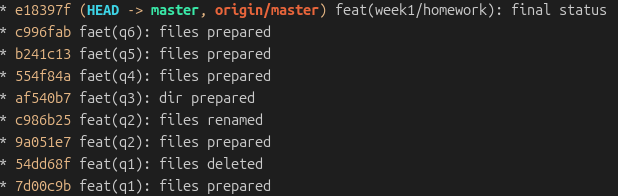
\includegraphics[width=0.8\textwidth]{figures/homework_commit.png}
        \caption{课后作业commit记录}
        \label{fig:homework_commit}
      \end{figure}
    
  \section{解题感悟}
    本次实验报告涵盖了系统开发工具基础的多个方面，包括文件操作、日志分析、版本控制以及 LaTeX 文档编写。通过实际操作，我不仅巩固了对基本命令的理解，还学会了如何处理复杂的任务，如合并冲突和交叉引用。在完成课后作业时，我进一步提升了自己的问题解决能力，尤其是在使用 Shell 脚本和 Git 工具方面。总的来说，这次实验让我对系统开发工具有了更深入的认识，并为今后的学习和工作打下了坚实的基础。 

\end{document}